\documentclass[dakotalogo]{dakota-article}


\usepackage{pifont}% allow use of arrows for items
\newcommand{\myitem}{\item[\color{darkblue}\ding{228}]}


\funding{This work was supported by ASC software. Sandia National Laboratories is a multi-program laboratory managed and operated by Sandia Corporation, a wholly 
owned subsidiary of Lockheed Martin Corporation, for the U.S. Department of Energy's National Nuclear Security 
Administration under contract DE-AC04-94AL85000.}
\def\mytitle{Surrogates: Emulating computer simulations}
\title{\mytitle}
\shorttitle{Dakota Technical Design Document}
\date{March 2017}
\def\mycorauthor{John D. Jakeman}
\corauthor{\mycorauthor}
\coremail{jdjakem@sandia.gov}

\def\SNL{Sandia National Laboratories, Albuquerque, New Mexico, USA }
%\def\corauthor{{\color{darkblue} Correspondence author}. \SNL   (jdjakem@sandia.gov)}

\shortauthor{Adams, Hooper, Jakeman, Rushdi}
\author{B. Adams\thanks{\SNL}, R. Hooper\samethanks[1], \mycorauthor\samethanks[1], A. Rushdi\samethanks[1]}

\setlength{\headheight}{21pt}%
\begin{document}
\pagestyle{myheader}
\maketitle
\section{Introduction}
\subsection{Purpose}
This library will provide a suite of algorithms for emulating expensive computer simulations.

\subsection{Scope}
This library will replace the existing surrogate tools in Dakota and enrich these existing tools with additional state of the art surrogates and algorithms.

\subsection{Overview}
This library will consist of 5 main software components visible to the user at the highest level of abstraction:
\begin{itemize}
\myitem Function - A class, from which surrogates is derived whose interface represents the mathematical properties of a $C_2$ continous function, e.g supports evaluation of values, gradients and Hessians. evaluated 
\myitem Variables - A class defining the properties of the function variables, e.g. probability distribution, ranges, etc. We will support all current Dakota Variable types in addition to blocks of correlated variables whose distribution is known, data-based-variables whose distribution is computed from data, and compositions of all variables.
\myitem Data - A class to store data returned by function and the associated samples of the function variables. This class will also contain fault information. We must provide modules that convert simple structures such as matrices and vectors of samples and values into this class. 
\myitem SurrogateFactory - A factory to construct a surrogate/approximation. Typical workflow will be generate a set of samples, evaluate function at those samples and build approximation. This call structure can be repeated iteratively to build up surrogates adaptively. We will also support the use and enrichment of archived data. This factor will support typical Dakota use-cases, however uses will be easily able to develop and add there own methods for building surrogates. 
\myitem SurrogateAnalyzer - A factory for running various types of analysis on surrogate models, e.g. compute moments, sobol indices, etc. If certain surrogates support fast operations to compute these values, e.g. PCE can compute mean and variance analytically these specialized functions will be envoked, but other wise a default will be called.
\end{itemize}
Currently the above notions of function and surrogate builders and analysis are heaverly intertwined in Dakota. Our design will allow these distinct components to be separated. This will allow surrogates to become a standalone part of the dakota Model hierarchy and surrogate analyzers to become lightweight Dakota Iterators.

\subsection{Requirements}
The following is a list of requirements
\begin{itemize}
\myitem User flexibity. Design must support 'push-button' users that want hired wired behavior and power users that wish to develop their own surrogate methods or expose low-level functionality.
\myitem Serialization of surrogates - Ability to save and load surrogate objects
\myitem Python interface - be able to call both high-level and low-level functions using Python. 
\myitem Gaussian Process consolidation - Consolidate GP methods in Dakota. Extend GP to include estimation of hyper-parametersa and use PCE trend function.
\myitem Surrogates for multiple QOI - Build a single surrogate for multiple QOI. Allow for composition of surrogate types.
\myitem Exending variable class - Support all Dakota variable types as well as blocks of correlated variables whose distribution is known, data-based-variables whose distribution is computed from data, and compositions of all variables. Retirement of AleatoryDistParams in Dakota.
\myitem Simple approximation classes. Separation of approximation and the code used to construct it. Particularly relevant in Pecos. RegressOrthogPolynomial contains PCE object but also regression methods used to build the PCE. Similarly for Sparse grids need to seperate approximation, either lagrange polynomials or PCE, from refinement tools For example, split current subspaces which are part of approximation from active subspaces being considered for refinement which should only been known to sparse grid builder 
\myitem Function Data. The function data class should have no notion of active and stored data we shold just use indexing to access the data needed. 
\end{itemize}


\section{Design}
\subsection{High-level interface}
The following is an example of the typical workflow used to build a surrogate
\begin{codelisting}[]{Construct Surrogate Demonstration}
  
// Configure options used to build surrogate
Teuchos::ParameterList factor_opts;
factory_opts.set(function, "target function");
factory_opts.set(data, "optional archived data");
factory_opts.set(PCE, "approximation type");
factory_opts.set("regression", "construction method");
//factory_opts.set("adapted-regression", "construction method");
factory_opts.set("OMP", "regression solver");
factory_opts.set("random", "sample type");
//factory_opts.set("optimal", "sample type");

// Build surrogate
Teuchos::RCP<Approximation> approx = SurrogateFactory(factory_opts);

// Analyze surrogate
Teuchos::ParameterList analyzer_opts;
analyzer_opts.set(MOMENTS, "analysis type");
Teuchos::RCP<AnalyzerMetrics> result = SurrogateAnalyzer(approx, analyzer_opts);

// Print metrics
std::cout << "Mean: " << result.get("mean") << std::endl;
std::cout << "Variance: " << result.get("variance") << std::endl;
  
\end{codelisting}

\subsection{Surrogate Interface}
We will use a factory pattern to build a surrogate. The Surrogate factory will call lower level factories which are specific to each type of approximation. Approximation types can be added at these levels without the call to surrogate factory being modified. These new types can just be created by passing appropriate options via {\texttt Teuchos::ParameterList}.
\begin{codelisting}[]{Surrogate Factory}
enum ApproxType {PCE,GP};
Teuchos::RCP<Approximation> surrogate_factory(const Teuchos::ParameterList opts){
  ApproxType approx_type = opts.get<ApproxType>("approximation type");
  switch (approx_type){
    case PCE : {
      return PCEFactory(opts, approx);
    }
    case GP : { 
      return GPFactory(opts, approx);
    }
    default : {
      throw(std::runtime_error("Incorrect approximation type"));
    }
  }
}
\end{codelisting}

\subsection{Surrogate Analyzer}
The surrogate analyzer will be implemented using a factory pattern. The analyzer will support various types of analysis on surrogate models, e.g. the computation of moments, sobol indices, etc. If certain surrogates support fast operations to compute these values, e.g. PCE can compute mean and variance analytically these specialized functions will be envoked, but other wise a default will be called.
\begin{codelisting}{Surrogate Analyzer}
enum AnalysisType {MOMENTS,SOBOL_INDICES};
Teuchos::RCP<AnaylzerMetrics> surrogate_anaylzer_factory(const Teuchos::ParameterList opts, Approximation &approx){
  AnalysisType analysis_type = opts.get<AnalysisType>("analysis type");
  switch (analysis_type){
    case MOMENTS : {
      RealVector means, variances;
      Teuchos::ParameterList moment_opts;
      moment_opts.set(false, "compute mean");
      moment_opts.set(false, "compute variance");
      if (!approx.get("mean",means))
      // if specialized method does not exist use default
      moment_opts.set(true, "compute mean");
      if (!approx.get("variance",variances))
      // if specialized method does not exist use default
      moment_opts.set(true, "compute variance");
      compute_moments_using_sampling_carlo(
      approx,moment_opts,means,variances)
      break;
    }
    case SOBOL_INDICES : { 
      RealMatrix sobol_indices;
      if (!approx.get("sobol_indices",sobol_indices))
      // if specialized method does not exist use default
      // opts can contain options like restricted indices
      compute_sobol_indices_using_sampling(approx,opts,sobol_indices);
      break;
    }
    default : {
      throw(std::runtime_error("Incorrect approximation type"));
    }
  }
}
\end{codelisting}

\subsection{Approximations}
Approximations will all be derived from a base function class. The interface of the function class will be restricted to only those functions that represents the mathematical properties of a $C_2$ continous function, e.g supports evaluation of values, gradients and Hessians. Each approximation will only contain the methods relevant to its construction, e.g. PCE has {\texttt build\_basis\_matrix} and {\texttt set\_coefficients} and GP has {\texttt build\_correlation\_matrix} and {\texttt set\_correlation\_lenghts}.

The basic approximation class hierarchy is depicted in Figure~\ref{fig:approx-class-hierarcy}. This hierarchy will be extended as additional approximation types are added.

\begin{figure}[htb]\centering
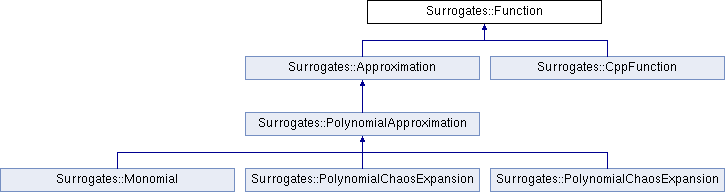
\includegraphics[width=0.7\textwidth]{classSurrogates_1_1Function.png}
\caption{Function class hierarchy.}
\label{fig:approx-class-hierarcy}
\end{figure}  

\subsubsection{Function base class}

Here we describe the abstract base class representation of a function $f(x)$ for a multivariate variable x.
Functions derived from this class can either be $C_0, C_1$ or $C_2$
 continuous. Regardlesd of the function regularity any derived class must
implement value(), $C_1$ functions must implement gradient() and jacobian()
and $C_2$ functions must implement hessian().

To avoid complexity of the function hierarchy we do not create seperate classes
for  $C_0, C_1$ and $C_2$ functions but rather only implement the
functions necessitated by the function regularity. All other functions must
raise an exception if called (these exceptions are implemented in this base
class)
\begin{figure}[htb]\centering
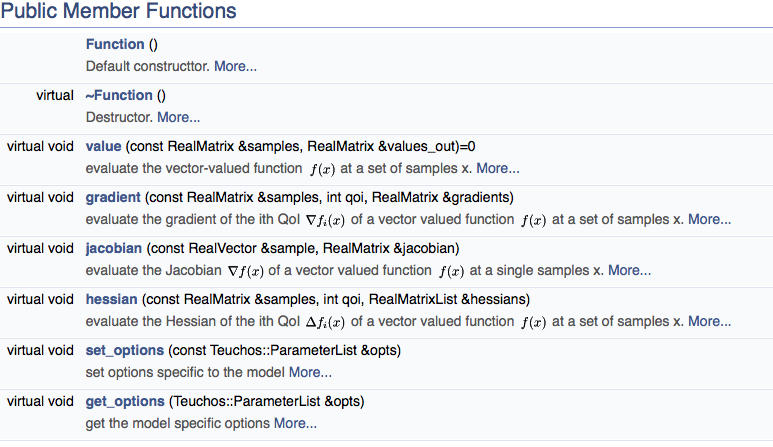
\includegraphics[width=0.7\textwidth]{function-class-members.png}
\caption{Function base class member functions.}
\end{figure}

QUESTION: Do we have functions for value, gradient, hessian or do we
have a function value(samples,opts) where opts specifies what of the
three data to return.

\subsection{Variables}
Variables is a class defining the properties of the function variables, e.g. probability distribution, ranges, etc. There is almost no functionality in the base class except {\texttt num\_vars}. The rest of the functionality is implemented in the derived class and variable transformations or approximations which use the derived class must know what additional functions are implemented. An example of a variable class is shown in Figure~\ref{fig:bounded-vars-class}. 

\begin{figure}[htb]\centering
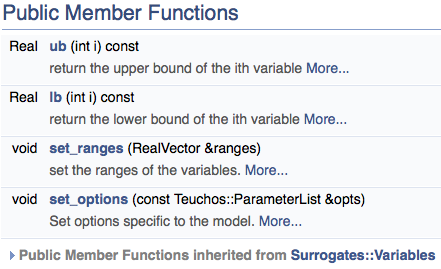
\includegraphics[width=0.7\textwidth]{bounded-vars-members.png}
\caption{Example of a variables class.}
\label{fig:bounded-vars-class}
\end{figure}  

\subsubsection{Variable Transformations}
Surrogates will sometimes the users provided variables to be mapped to a set of variables that the approximation can use. E.g a PCE requires variables on canonical domains such as Uniform on $[-1,1]$. These mappings are peformed by variable transformations. An example implementation for an affine transformation of bounded variables is shown below.
\begin{codelisting}{Example of variable transformation code}
void AffineVariableTransformation::
map_samples_from_user_space(const RealMatrix &samples, 
RealMatrix &transformed_samples) const {
  int num_vars = boundedVars_->num_vars();
  if ( samples.numRows() != boundedVars_->num_vars() )
    throw( std::runtime_error("Samples have incorrect number of random variables") );

  int num_samples = samples.numCols();
  transformed_samples.shapeUninitialized(num_vars, num_samples);
  for ( int j=0; j<num_samples; j++ ){
    for ( int i=0; i<num_vars; i++ ){
      transformed_samples(j,i) =
	(samples(i,j)+1)/2.*(boundedVars_->ub(i)-boundedVars_->lb(i))+boundedVars_->lb(i);
    }
  }
}
\end{codelisting}

Here is an example of using a variable transformation
\section{Approximation Builders}
The approximation factories call approximation builders. An example of
how a builder may work is given below. This builder consists of two
steps defining the approximation and the sampling the function and
solving for its coefficients using regression. builders may call
other builder in an inner loop. For example we may wish to iteratively
add samples. In which case we would call this builder in an inner loop
until an error estimate reaches a desired level of accuracy. In the
example below we pass in a function but we could also pass in existing data.
\begin{codelisting}{Example of a surrogate builder}
// Define the function variables
  RealVector ranges;
  define_homogeneous_ranges(num_vars, 0., 1., ranges);
  Teuchos::RCP<Variables> variables(new BoundedVariables());
  Teuchos::rcp_dynamic_cast<BoundedVariables>(variables)->set_ranges(ranges);

  // Define the variable transformation. Need to decide if a seperate
  // transformation should exist for approximation and for mapping samples
  // generated. For example approximation accepts samples in user x-space
  // but operates in a standardized u-space. But sample generator produces
  // samples in (possibly another standardized space) and must map these to
  // x-space, or even to approximation u-space.
  Teuchos::RCP<VariableTransformation> var_transform(new AffineVariableTransformation());
  var_transform->set_variables(variables);

// Initialize the approximation
  Teuchos::ParameterList monomial_opts;
  monomial_opts.set("max_total_degree",degree,
		    "max degree of total-degree polynomial space");
  monomial_opts.set("num_qoi", num_qoi, "number of quantites of interest.");
  Monomial monomial;
  monomial.set_options(monomial_opts);
  monomial.set_variable_transformation(var_transform);
  IntMatrix basis_indices;
  compute_hyperbolic_indices(num_vars, degree, 1., basis_indices);
  monomial.set_basis_indices(basis_indices);

  // Generate the approximation coefficients using a regression based method
  Teuchos::ParameterList regression_opts;
  regression_opts.set("regression type",SVD_LEAST_SQ_REGRESSION);
  regression_opts.set("num_samples",num_samples);
  regression_opts.set("sample_type","probabilistic_MC");
  RegressionBuilder builder;
  builder.set_target_function(model);
  builder.build(regression_opts, monomial);
\end{codelisting}
QUESTION: DO we pass in target function and any data through
ParameterList opts or through member functions?
\subsection{Regression methods}
For a given approximation type, there are a number of ways one might want
to construt the approximation. For example we can use different types
of regression to build a PCE, neural net etc, or we may want to build
a pseudo spectral pce using different types of quadrature. In these
cases we need factories to choose the builder sub-component,
e.g. least squares or l1 minimization for regression based pce, or
monte carlo or sparse grid quadrature for pseudo spectral pce.
An example of such builders is given below.
\begin{codelisting}[]{Example builder for regression based
    approximations}
  // Generate samples to build approximation
  int num_samples = opts.get<int>("num_samples");
  std::string sample_type = opts.get<std::string>("sample_type");

  // Create mc sampler and pass in sample type.
  // For now hack support for uniform mc sampler
  RealMatrix samples;
  int seed = 1337;
  Teuchos::RCP<VariableTransformation> var_transform =
    approx.get_variable_transformation();
  generate_uniform_samples(approx.num_vars(), num_samples, seed,
			   *var_transform, samples);
    
  // Evaluate the function at the build samples
  RealMatrix values;
  targetFunction_->value(samples, values);
    
  //\todo consider having opts have multiple parameterLists
  //each associated with a particular aspect of build
  //e.g. opts = (sample_opts, regression_opts)
  PolynomialApproximation& poly_approx = 
    dynamic_cast<PolynomialApproximation&>(approx);
    
  // Generate matrix of the linear system to be used in
  // regression solve
  RealMatrix basis_matrix;
  poly_approx.generate_basis_matrix(samples,basis_matrix);
    
  // Solve regression problem to get coefficients
  Teuchos::RCP<LinearSystemSolver> solver =
    regression_solver_factory(opts);
  RealMatrix coeffs, metrics;
  solver->solve(basis_matrix, values, coeffs, metrics, opts);
  
  // Set the approximation coefficients
  poly_approx.set_coefficients(coeffs);
\end{codelisting}
The solvers inheritance diagram is depicted in
Figure~\ref{fig:regresion-solver-inheritance}. The hierarchy lets each
class define specialized implementations of things like cross
validation. Sparse solvers have a default implementation of iterative
reweighting which they can call, the definition of this function DOES
NOT exist in the base class.
\begin{figure}[htb]\centering
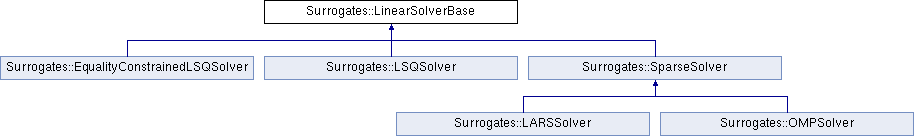
\includegraphics[width=0.7\textwidth]{classSurrogates_1_1LinearSystemSolver.png}
\caption{The regression solver hierarchy.}
\label{fig:regresion-solver-inheritance}
\end{figure}
Specialization of sparse solver is shown in
Figure~\ref{fig:sparse-solver-members}
\begin{figure}[htb]\centering
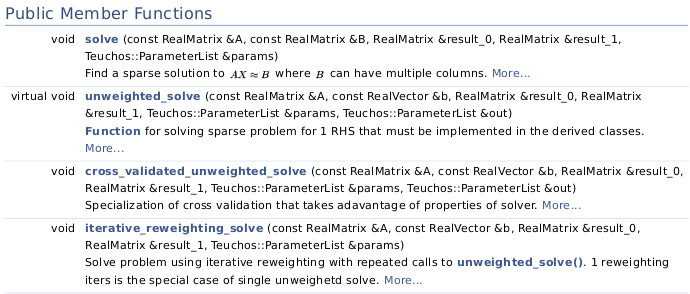
\includegraphics[width=0.7\textwidth]{sparsesolverclass.jpeg}
\caption{Sparse solver member functions. Only solve exists in baseclass}
\label{fig:sparse-solver-members}
\end{figure}
\section{Integration with Dakota}
Currently the notions of Approximation (DataFitSurrogate) and surrogate builders and analysis are heaverly intertwined in Dakota. Our design will allow these distinct components to be separated. This will allow Approximation to become a standalone part of the dakota Model hierarchy and surrogate analyzers to become lightweight Dakota Iterators.



\section{Variables}

The Variables class is intended to encapsulate the creation, augmentation
and realization of random variables.  Single variables are characterized
by such properties as probability distribution, ranges, hyperparameters,
etc. A base class provides only the bare minimum via a {\texttt num\_vars}
attribute and a pure virtual {\texttt realize()} method. The rest of
the functionality is implemented in the derived classes and require that
variable transformations or approximations which use the derived classses
to know what additional functions are implemented. (These could change.)

\subsection{Requirements}

The following are requirements the the Variables class must support in any design and
implementation:

\begin{enumerate}
  \item Functionality and use cases currently supported in the
        Pceos::RandomVariable class must be preserved.
  \item Appropriate leveraging of Boost's stastical distributions should
        be preserved.
  \item Consistent and performant extensions to available distributions
        should be added as needed, eg distributions based on underlying
        user-supplied data.
  \item Extensions to multivariables ranging in type from iids to
        aggregations of varying distributions should be implemented
        in a way that preserves good performance while scaling up to
        high dimensions.
  \item Correlations among variables should be able to be specified at
        construction or updated thereafter.
  \item Transformations (including inverse when possible) should be supported
        with checks for appropriateness and consistency.
  \item Where appropriate transformations should support distributions, e.g.
        return a new distribution, and realizations, e.g. map realizations from
        one underlying distribution to a value coreresponding to another distribution.
  \item The previous transformation reuirements should apply to multivariables
        irespecting correlations where appropriate.
  \item Variables (single and multiple) should be able to be serialzied for the 
        purpose of export/import, e.g. for supporting restart capabilitiy
\end{enumerate}



\subsection{Creation APIs}

The following examples illuatrate candidate APIs for creating single
and multi-variable instances.

\begin{codelisting}{Example of single variable construction}
  Teuchos::ParameterList & var_opts;
  var_opts.set("distribution", "Uniform");
  var_opts.set("alpha", "-1.0");
  var_opts.set("beta" , "1.0");
  auto sVar = VariableFactory::create<>( var_opts );
\end{codelisting}


\begin{codelisting}{Example of creating an independent IID multivariable}
  Teuchos::ParameterList & var_opts1;
  var_opts1.set("distribution", "Uniform");
  var_opts1.set("alpha", "-1.0");
  var_opts1.set("beta" , "1.0");
  auto sVar = VariableFactory::create<>( var_opts1 );

  // Create a 10-dim uniform(-1.0, 1.0) iid multivariable
  auto iidVar = VariableFactory::IID( sVar, 10 );
\end{codelisting}


\begin{codelisting}{Example of creating an independent joint multivariable}
  Teuchos::ParameterList & var_opts1;
  var_opts1.set("distribution", "Uniform");
  var_opts1.set("alpha", "-1.0");
  var_opts1.set("beta" , "1.0");
  auto sVar1 = VariableFactory::create<>( var_opts1 );

  Teuchos::ParameterList & var_opts2;
  var_opts2.set("distribution", "Standard-Normal");
  auto sVar2 = VariableFactory::create<>( var_opts2 );

  auto mVar = VariableFactory::Joint( std::vector<VariableBase> {sVar1, sVar2} );
\end{codelisting}


\subsection{Sampling APIs}

The following examples demonstrate how to obtain variates (realizations
of random variables).

\begin{codelisting}{Example of variable realization (sampling)}
  auto sample = mVar.realize(); // would return a vector<Real> of size 2 
                                // using the multivariable creation  example
\end{codelisting}


\subsection{Modification APIs}

The following examples demonstrate how to reset existing instances
of random variables and provide a possible means of efficient variate
realizations for large dimension variables.

\begin{codelisting}{Resetting an existing uniform variable configuration}
  auto suVar = VariableFactory::create<>( var_opts );

  std::cout << "Value 1 = " << suVar.realize() << std::endl;
  auto old_config = suVar.param();
  suVar.param(Surrogate::UniformDistribution<>::param_type {-1.0, 1.0});
  std::cout << "Value 2 = " << suVar.realize() << std::endl;
  suVar.param(old_range);
  std::cout << "Value 3 = " << suVar.realize() << std::endl;
\end{codelisting}




% \begin{figure}[htb]\centering
% %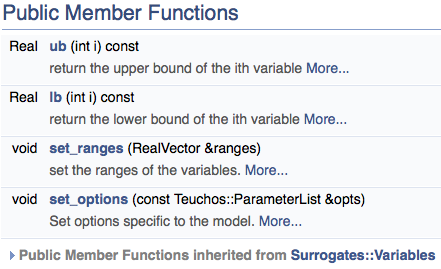
\includegraphics[width=0.7\textwidth]{bounded-vars-members.png}
% \caption{The relationship of surrogate classes to the Dakota class hierarchy}
% \label{fig:bounded-vars-class}
% \end{figure}  
\end{document}

%%% Local Variables:
%%% mode: latex
%%% TeX-master: t
%%% End:
